\chapter[Validating KomaMRI]{Validating KomaMRI}
\label{ch:validating-komamri}

KomaMRI is the simulation environment that all RL agents in this project
interact with, so simulator validation is a prerequisite for every result in
this project. Although KomaMRI is a peer-reviewed, open-source, and actively
maintained MRI simulation framework~\cite{komaMRI:23}, the validation
experiments in this project found two floating-point time-discretisation
failures.
Both were triggered by long cumulative sequence time. The failures were reduced
to minimal reproducers and fixes were contributed upstream:
\href{https://github.com/JuliaHealth/KomaMRI.jl/issues/779}{issue \#779} /
\href{https://github.com/JuliaHealth/KomaMRI.jl/pull/780}{PR \#780}, now
merged, and
\href{https://github.com/JuliaHealth/KomaMRI.jl/issues/788}{issue \#788} /
\href{https://github.com/JuliaHealth/KomaMRI.jl/pull/789}{PR \#789}, open at
the time of writing.

This work is part of A1, the validated digital twin and simulator pipeline, and
directly addresses C1: simulator validation for qMRI. For A1, the key
contribution is the validation of the simulation pipeline rather than the
upstream reports alone. The two failures were reduced to minimal reproducers, traced to
specific floating-point timing mechanisms, fixed upstream, and then verified by
recovering the phantom's known $T_1$ values in the full qMRI pipeline.

\section{KomaMRI simulation model}
\label{sec:komamri-simulation-model}

KomaMRI simulates the magnetization of each spin of a \texttt{Phantom} for
variable magnetic fields given by a \texttt{Sequence}~\cite{komaMRI:23}. All
\texttt{Phantom} objects used in this project were produced by
\texttt{MRISystemPhantom.jl}. Each \texttt{Phantom} is a cloud of spin
isochromats: groups of nearby nuclei that are assumed to share a single
position $(x,y,z)$ and one set of tissue parameters
$(T_1,T_2,T_2^*,\rho,\Delta\omega)$. Here $\rho$ is proton density and
$\Delta\omega$ is off-resonance: the offset of that isochromat's Larmor
frequency from the nominal scanner frequency. Each isochromat is therefore
represented by a magnetisation vector $(M_x,M_y,M_z)$ evolving according to the
Bloch equations.

The user-facing interface is:

\begin{verbatim}
raw = simulate(phantom, sequence, scanner; sim_params)
\end{verbatim}

Here \texttt{scanner} defines the scanner hardware used to play the sequence.
In these experiments it is an idealised hardware model: eddy currents and field
inhomogeneities are not modelled. This means RF pulses are treated as exact,
although in reality a 180$^\circ$ refocus pulse can vary by a couple of degrees
across the excited volume.

A \texttt{Sequence} is made up of RF pulses, which rotate the magnetisation
vector, as well as gradients, delays, and ADC readouts. Internally,
\texttt{simulate} represents the continuous sequence on a discretised time
grid. Gradient events use a time step $\Delta t$, while RF pulses are sampled
more finely using $\Delta t_\mathrm{rf}$. These time points are then split into
blocks. In excitation blocks, where RF is active, KomaMRI integrates the full
magnetisation rotation. In precession blocks, where RF is off, the update
reduces to relaxation and phase accrual, which can be computed analytically
with exponentials and is cheaper to evaluate. At each ADC sample, the simulator
sums the transverse magnetisation over all spins to form the complex received
signal $\mathrm{sig}[t]$.

The key computational assumption is that spins evolve independently and only
interact through the final signal sum. This is a standard MRI simulation
approximation and is less restrictive than the hardware idealisations above. It
is also what makes KomaMRI practical for this project: spins can be partitioned
across CPU threads or GPU kernels, then summed only at the receiver. This
parallelism motivated the use of KomaMRI and helps overcome C2, the cost of
simulation. KomaMRI also models bulk $T_2^*$ decay rather than microscopic
spin-spin interaction. Overall, these are standard MRI simulator assumptions
that model the relevant physics to an acceptable error, so learned policies
should plausibly generalise to real hardware.

\section{Initial validation failure}
\label{sec:komamri-initial-validation-failure}

The first validation test was deliberately simple. With no added noise, the
test simulated an inversion-recovery sweep across the 14 $T_1$ spheres and fitted
the standard monoexponential recovery model:

\[
M_z(\mathrm{TI}) = M_0 \left(1 - 2e^{-\mathrm{TI}/T_1}\right).
\]

In a noise-free digital phantom, this should be almost exact. Instead, the
fitted $T_1$ values had a mean absolute percentage error (MAPE) of 39.4\%,
with some spheres close to 100\% error. The recovery points did not lie on a
monoexponential curve. Either the simulator, sequence, reconstruction, or
fitting pipeline was wrong, or there was relevant MRI physics not captured by
the simple recovery model.

\begin{figure}[t]
\centering
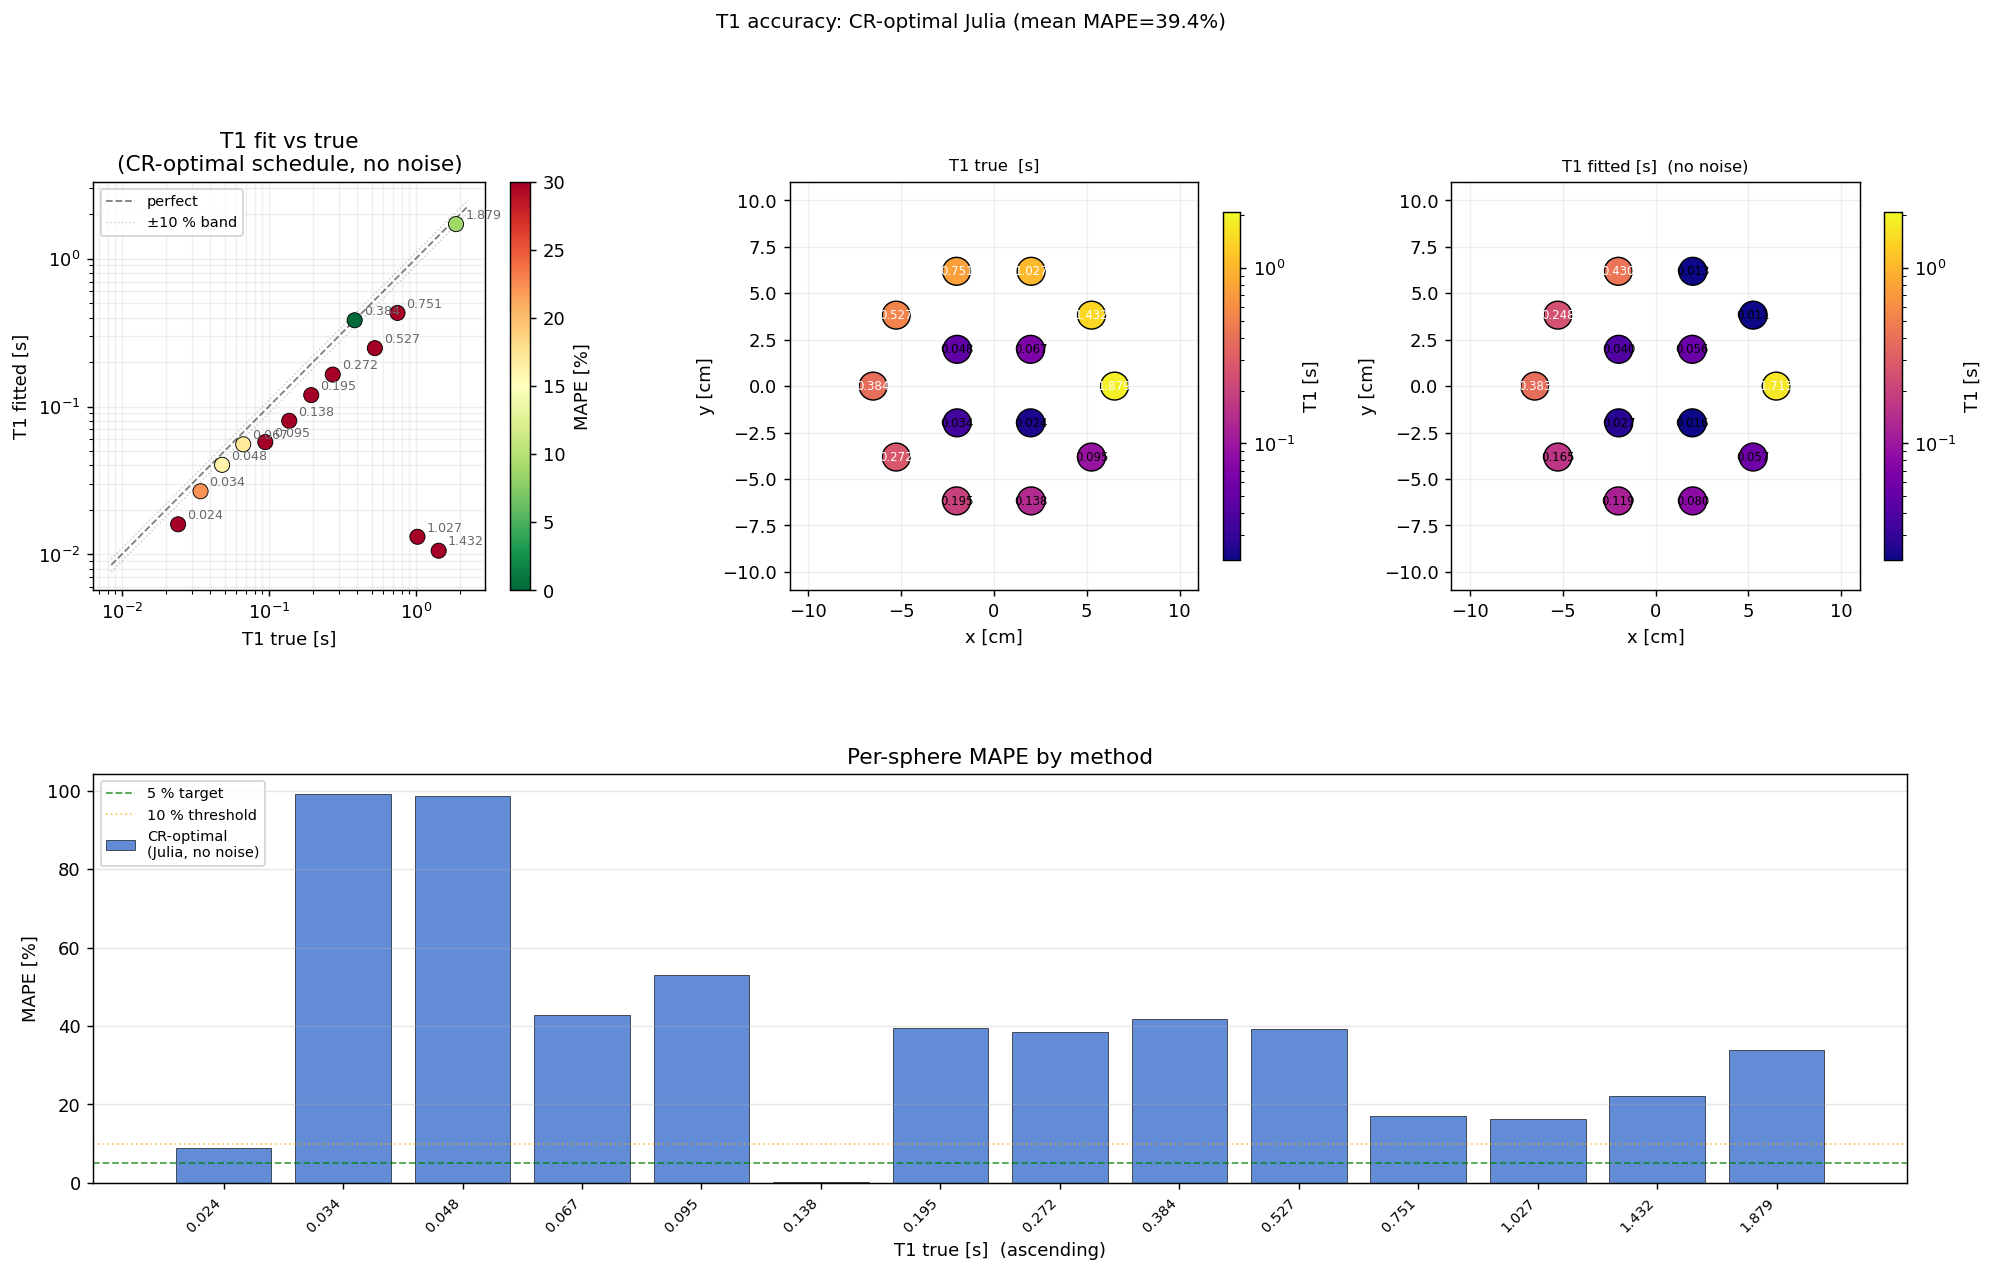
\includegraphics[width=0.72\linewidth]{imgs/komaMRI/buggy_t1_fit_vs_true.png}
\caption{Noise-free $T_1$ recovery before the KomaMRI fixes. The fitted values
should lie on the diagonal. Instead the mean MAPE is 39.4\%, with only two out
of the 14 spheres in the $\pm$10\% band.}
\label{fig:komamri-buggy-t1-fit}
\end{figure}

\begin{figure}[t]
\centering
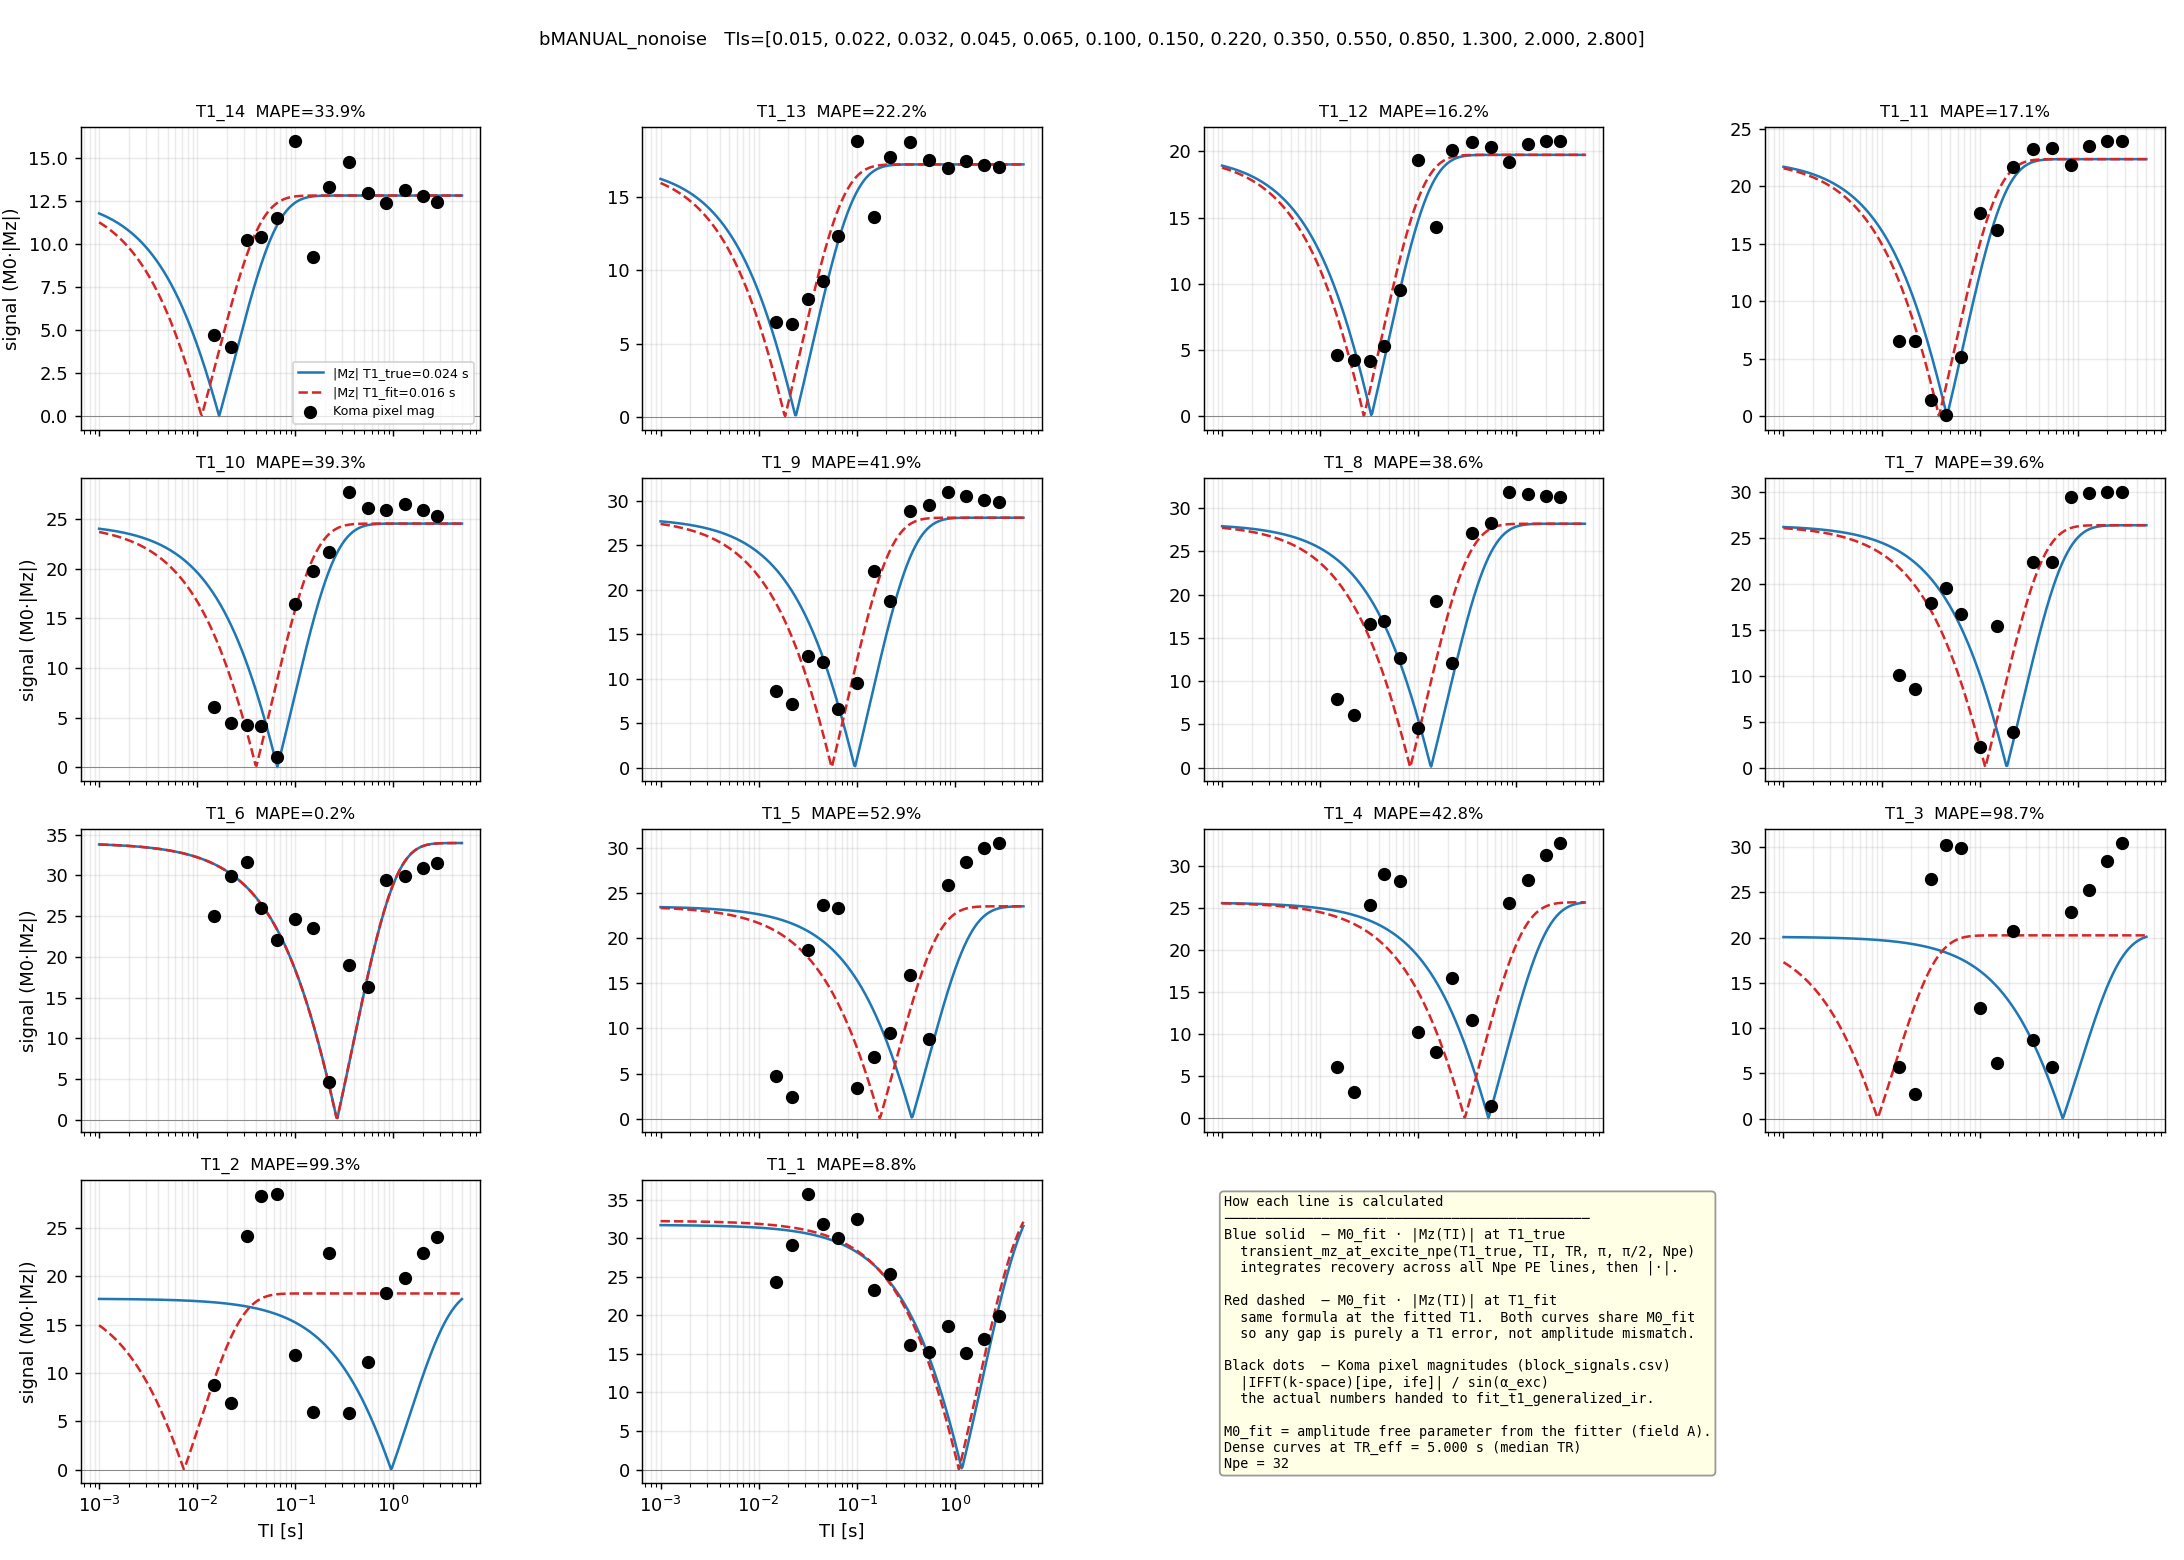
\includegraphics[width=0.9\linewidth]{imgs/komaMRI/buggy_recovery_curves_koma.png}
\caption{Recovery points before the KomaMRI fixes. The simulated samples do
not lie on the best-fit monoexponential curves. The deviation is structured,
not random, so it points to a repeatable simulation or analysis error.}
\label{fig:komamri-buggy-recovery-curves}
\end{figure}

The first step was to rule out plausible MRI explanations. Imperfect transverse
spoiling was the most likely candidate: residual $M_{xy}$ can survive one
shot, be refocused by later RF pulses, and contaminate the next echo. The
standard way to suppress this is to add spoiler gradients, typically around the
end of the shot and around refocusing pulses, to dephase any remaining
transverse magnetisation. However, when implemented this did not remove the
error; it changed mean MAPE from 39.4\% to 44.0\%. Increasing TR also made the
fit worse, even though longer recovery time should reduce both residual
transverse coherence and incomplete longitudinal recovery. This was the first
strong clue that the failure was driven by total simulated time, not by the
physical state at the start of each shot.

Reconstruction explanations were also tested. Hamming-window filtering and ROI
masking did not remove the error, making ordinary Gibbs ringing unlikely. A
phase-sensitive reconstruction was also checked to ensure the magnitude image
was not hiding a sign or phase convention error. These tests changed details of
the images, but not the failure mode.

The decisive diagnostic was to inspect k-space directly. Rather than showing
random fitting error, the measured k-space collapsed after a fixed amount of
simulated time, even though the acquisition should have remained symmetric.
This shifted the investigation away from missing MRI physics and toward the
simulator's handling of long absolute times.

\begin{figure}[t]
\centering
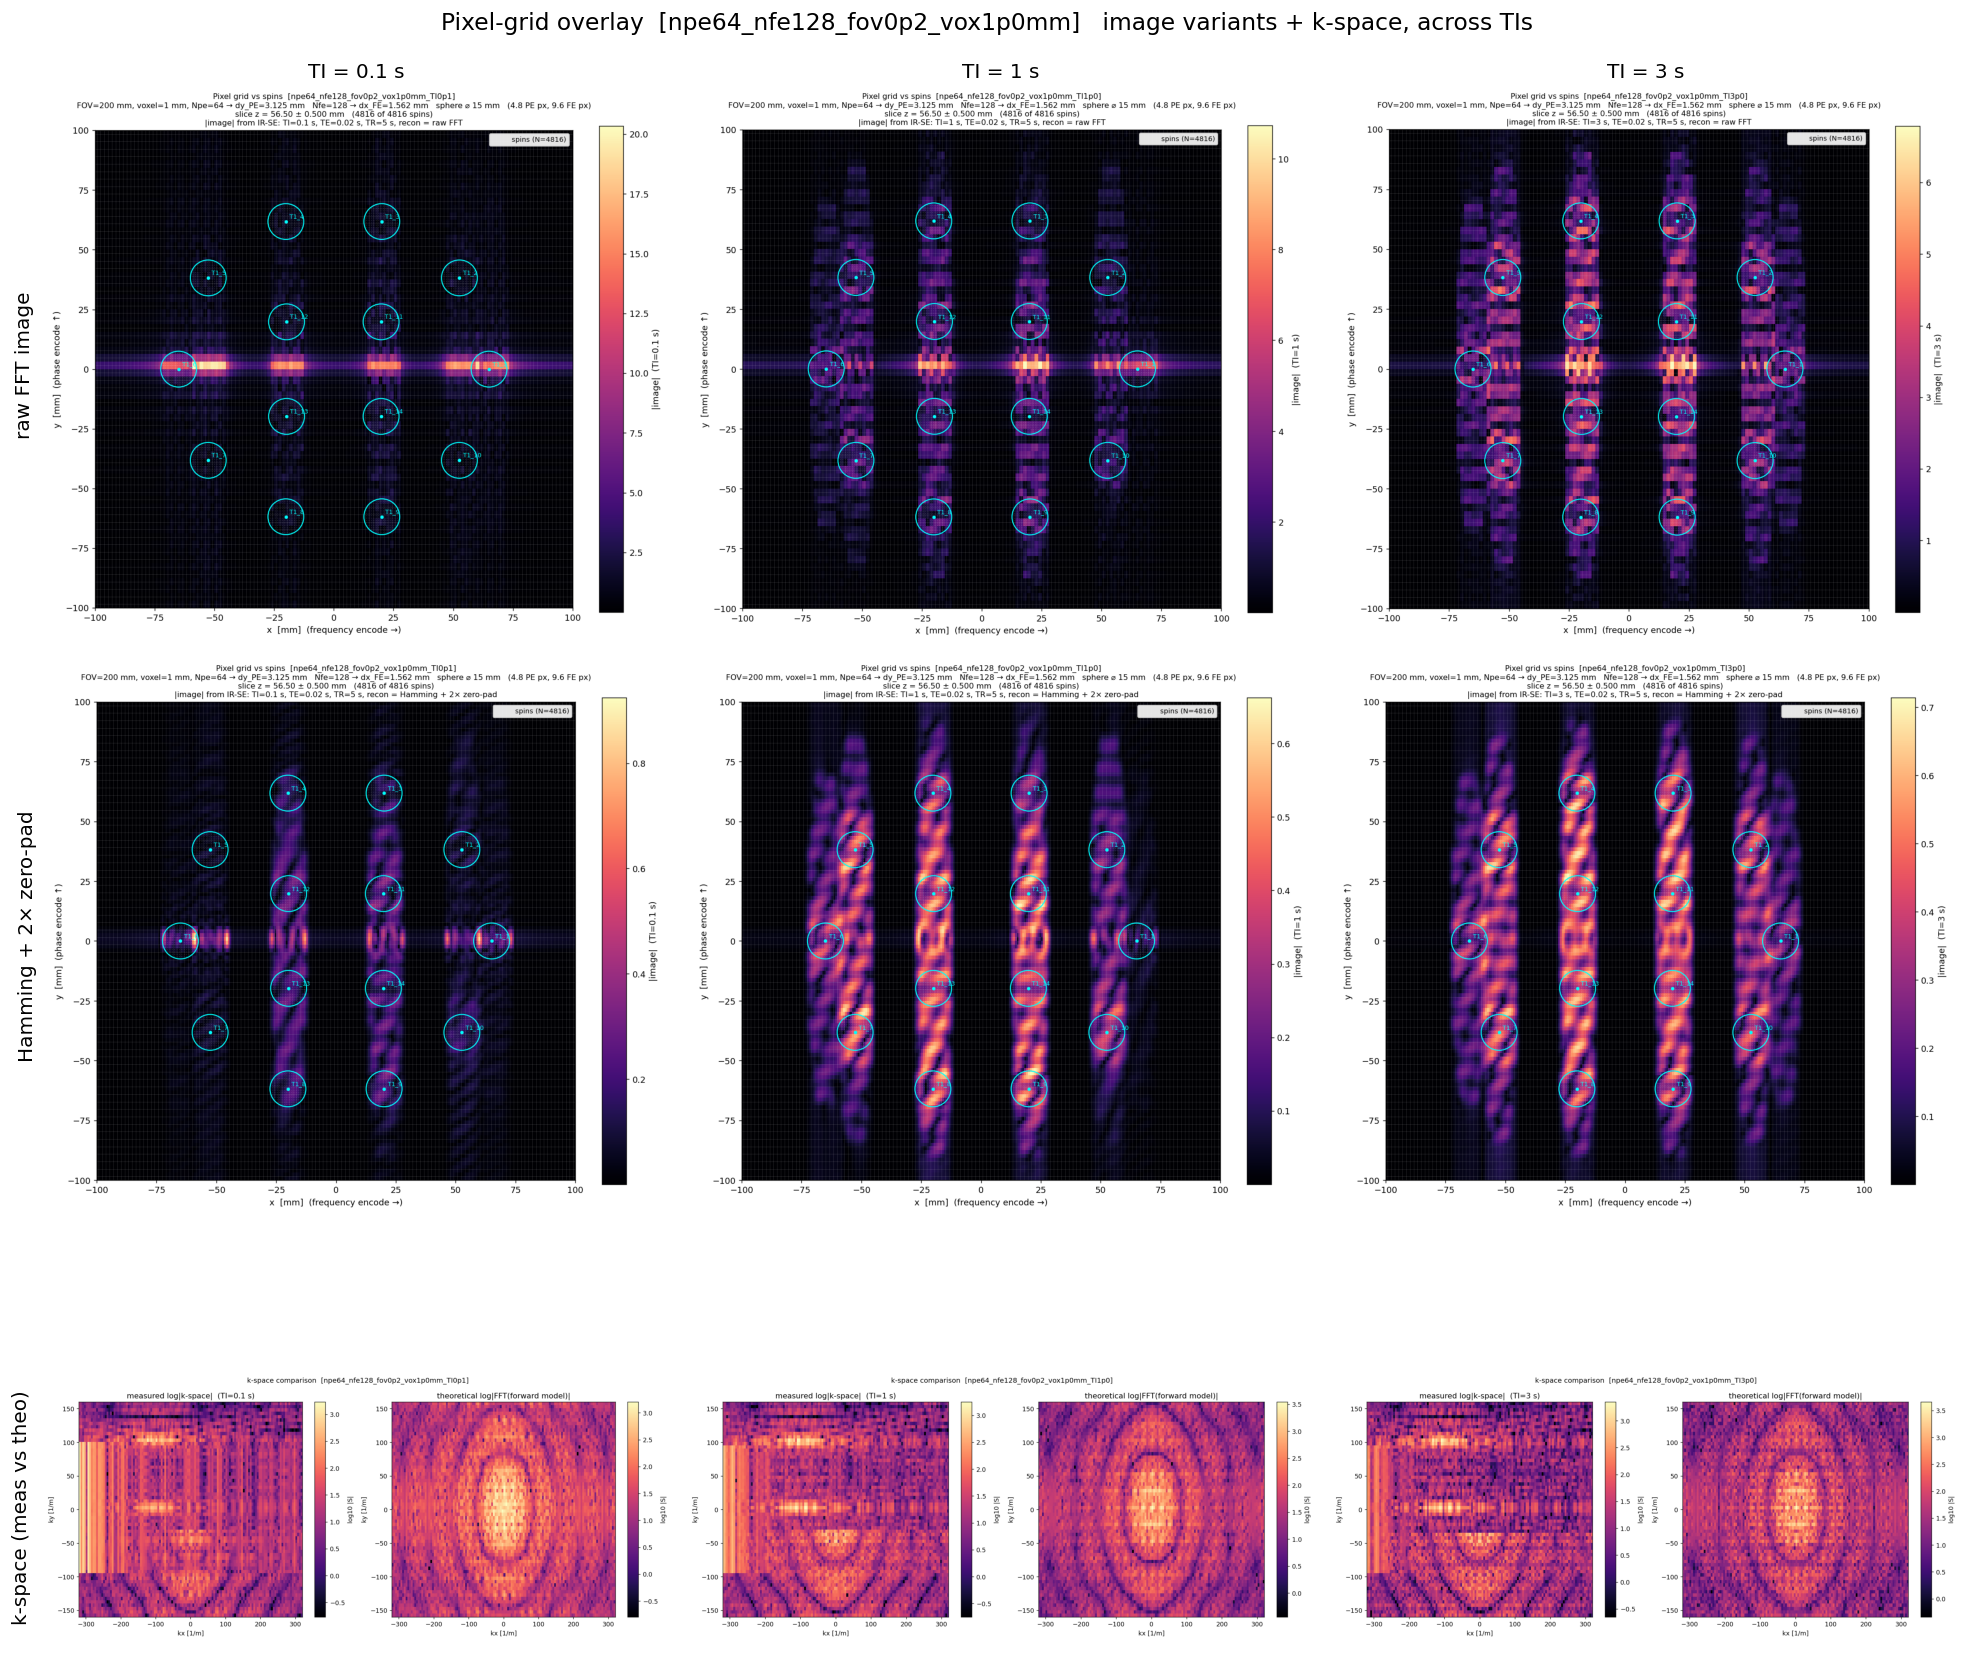
\includegraphics[width=0.95\linewidth]{imgs/komaMRI/buggy_pixel_grid_overlay.png}
\caption{Image-space symptom of the timing failure. The figure shows an IR-SE acquisition
at three inversion times (TI = 0.1, 1.0, and 3.0 s). The first row shows the
reconstructed image, the second row applies a Hamming window, and the bottom
row compares theoretical and measured k-space. Because the phase-encode
direction ($k_y$) is acquired shot by shot, moving along $k_y$ corresponds to
advancing in simulated time. The early phase-encode lines reconstruct
correctly, but later lines collapse into horizontal streaks after a fixed
cumulative time. This is too large and structured to be ordinary ringing, and
is not removed by the Hamming window. Generated by
\texttt{pixel\_grid\_overlay.jl}.}
\label{fig:komamri-buggy-pixel-grid}
\end{figure}

\section{RF edge marker collapse}
\label{sec:komamri-bug-1}

The first minimal reproducer was \texttt{koma\_bug\_minimal.jl}. It removed
the phantom geometry and reconstruction and repeated the same simple shot at
increasing absolute simulation times. The expected result was a constant
per-shot signal. Instead, sharp jumps appeared once cumulative simulated time
reached roughly 70--150 s. For example, with TR = 15 s the signal jumped at
shot 6 (\textasciitilde90 s) by 21\%; with TR = 8 s it jumped at shot 9
(\textasciitilde72 s) by 19\%; and with TR = 30 s it jumped at shot 4
(\textasciitilde120 s) by 21\%. This showed that the threshold was
time-driven, not shot-count-driven, and raised the next question: was KomaMRI
discretising the same RF pulse differently at large absolute time?

The RF-edge investigation revealed that the first failure was caused by the way
KomaMRI represents sharp RF edges on its simulation time grid. Tracing the RF
pulse discretisation led to \texttt{points\_\allowbreak from\_\allowbreak key\_\allowbreak times}, and then to the
edge-handling logic inside \texttt{get\_variable\_times}. In
\texttt{get\_variable\_times}, KomaMRI creates a small set of key times around
each RF pulse:

\begin{verbatim}
points_from_key_times(sort([t1, t1 + MIN_RISE_TIME, tc,
                            t2 - MIN_RISE_TIME, t2]); dt=Δt_rf)
\end{verbatim}

where \texttt{t1} and \texttt{t2} are the start and end of the pulse,
\texttt{tc} is the centre. KomaMRI encodes the sharp RF edge using a fixed
offset $\epsilon = 10^{-14}$ s, implemented as
\texttt{MIN\_RISE\_TIME}. The pair \texttt{(t1, t1 + MIN\_RISE\_TIME)}
is used to encode the rising edge of the
RF pulse. At \texttt{t1}, interpolation should return zero RF amplitude;
immediately after the edge, at \texttt{t1}+$\epsilon$, it should return
the full RF amplitude. This creates a near-discontinuous step while still
letting KomaMRI store the RF waveform using a small number of key points, with
interpolation filling in the values between them.

The problem is that $\epsilon$ is a fixed absolute time, but Float64 precision
is relative. The spacing between $t$ and the next representable Float64 number,
calculated by \texttt{eps(t)} in Julia, grows with the magnitude of $t$:
$\mathrm{eps}(t) \approx t\cdot2^{-52}$. Once
$\mathrm{eps}(t)/2 > \epsilon$, adding $\epsilon$ no longer produces a distinct
Float64 value. In practice this happens at about $t \geq 128$ s. Beyond this
point, \texttt{t1 + MIN\_RISE\_TIME == t1} bit-for-bit. The two key times that
should define the rising edge therefore collapse onto the same value. When the
time vector is sorted and deduplicated, one of them is removed.

The isolated test \texttt{koma\_bug\_isolate.jl} backed this up by asking
whether the same 1 ms RF pulse is converted into the same time points at
different absolute times:

\begin{wraptable}[7]{l}{0.38\textwidth}
\vspace{-\baselineskip}
\begingroup
\small
\setlength{\tabcolsep}{4pt}
\setlength{\columnsep}{10pt}
\centering
\begin{tabular}{rrrr}
\toprule
$t_0$ [s] & \texttt{nraw} & \texttt{nunique} & $\mathrm{eps}(t_0)$ \\
\midrule
0.0    & 24 & 23 & $5.0{\times}10^{-324}$ \\
3.0    & 24 & 23 & $4.44{\times}10^{-16}$ \\
67.0   & 24 & 23 & $1.42{\times}10^{-14}$ \\
99.0   & 24 & 23 & $1.42{\times}10^{-14}$ \\
200.0  & 26 & 21 & $2.84{\times}10^{-14}$ \\
1000.0 & 26 & 21 & $1.14{\times}10^{-13}$ \\
\bottomrule
\end{tabular}
\endgroup
\vspace{-0.5\baselineskip}
\end{wraptable}

The table shows the collapse directly: early pulses retain 23 unique time
points, but at $t_0=200$ s this falls to 21 as
$\mathrm{eps}(t_0)/2$ exceeds $\epsilon$. This confirms that the RF edge
markers have collapsed before simulation.

The collapsed points are not redundant: they represent the two sides of the RF
step. At \texttt{t1}, RF is zero; at \texttt{t1}+$\epsilon$, RF has reached
the pulse amplitude. Deduplicating them removes the edge, so the Bloch
integrator applies the wrong RF value for one full $\Delta t_\mathrm{rf}$
sample. For KomaMRI's default $\Delta t_\mathrm{rf}=5\times10^{-5}$ s and
$T_\mathrm{RF}=1$ ms, one missing sample is 5\% of the RF area. The
$\epsilon$-scale timing collapse therefore becomes a 5\% flip-angle error, producing a
20--25\% signal jump and later a biased $T_1$ fit.

The fix in \href{https://github.com/JuliaHealth/KomaMRI.jl/pull/780}{PR
\#780} made the edge markers adaptive:

\begin{verbatim}
next_time(t) = max(t + MIN_RISE_TIME, nextfloat(t))
prev_time(t) = min(t - MIN_RISE_TIME, prevfloat(t))
\end{verbatim}

\texttt{nextfloat} and \texttt{prevfloat} step to the adjacent representable
Float64 value, so the marker remains distinct even at large absolute time. At
small times the original spacing is preserved; at large times the marker
becomes one floating point step away rather than collapsing. This fixed the
first failure and was merged into KomaMRI.

\section{Closing knot collapse after time rebasing}
\label{sec:komamri-bug-2}

After \href{https://github.com/JuliaHealth/KomaMRI.jl/pull/780}{PR \#780} the
direct checks all passed: the isolated RF-edge script was stable to 1000 s, the
minimal multi-shot reproducer no longer drifted over the tested shots, and the
new RF-area regression test showed that the discretised pulse area matched the
expected trapezium area at large absolute time. The original failure mechanism
had genuinely been fixed.

However, the full no-noise $T_1$ validation was still inaccurate. Further
investigation revealed another fixed-$\epsilon$ collapse, but at a different
point in the time pipeline. KomaMRI also separates a block's closing knot, or
block edge, using the same fixed offset $\epsilon$ in block-relative time. This is
initially safe because the local block times are small (e.g. 1 ms RF pulses).
Later, however, \texttt{get\_variable\_times} and \texttt{get\_samples} rebase
these local times to absolute sequence time using \texttt{T0 .+ t}, where
\texttt{T0} is the absolute start time of the block. This creates the
same floating-point problem as before: at large values of \texttt{T0}, the
$\epsilon$ gap is below Float64 precision. The closing knot rounds onto the
block-end knot, the two times become bit-identical, and a later \texttt{unique!}
step removes one of them. The marker therefore disappears much later in the code
than where it was first created, which made this second failure harder to track
down.

The reproducer showed that the remaining timing error still mattered. It used one spin
and a gradient-free repeated inversion-recovery shot:

\begin{verbatim}
180 deg inversion -> TI -> 90 deg excitation -> one ADC sample -> TR delay
\end{verbatim}

Every shot is physically identical. At TR = 15 s, all 24 shots should return
the same signal. Instead, the first 17 shots were stable, shot 18 jumped by
52\%, and later shots settled to a new wrong plateau:

\begin{verbatim}
shot  1..17  (sim_time <= 255 s): |signal| = 0.476267 stable
shot 18      (sim_time  = 270 s): |signal| = 0.722479 +52%
shot 19..24  (sim_time >= 285 s): |signal| = 0.677159 new wrong plateau
\end{verbatim}

The fix in \href{https://github.com/JuliaHealth/KomaMRI.jl/pull/789}{PR
\#789} re-separates the closing knot after rebasing, when the correct
absolute-time spacing is known. In implementation terms, the closing knot is
moved to at most
$t_\mathrm{end}-\max(\epsilon,\mathrm{eps}(t_\mathrm{end}))$. The gap is
adaptive: it remains $\epsilon$ at small times, but widens
when Float64 spacing becomes larger. The re-separation is also idempotent: if
the closing knot is already distinct, it is left alone. The fix is applied at
each rebasing site: both RF sampling paths in \texttt{get\_samples}, and the
gradient timing path in \texttt{get\_variable\_times}. The latter also
re-applies an adaptive \texttt{\_strictly\_increasing\_knots!} check so
gradient knots remain ordered after rebasing. With this patch, the 24-shot
reproducer is flat and the KomaMRI tests still pass.

At the time of writing,
\href{https://github.com/JuliaHealth/KomaMRI.jl/issues/779}{issue \#779} is
merged upstream via
\href{https://github.com/JuliaHealth/KomaMRI.jl/pull/780}{PR \#780}.
\href{https://github.com/JuliaHealth/KomaMRI.jl/issues/788}{Issue \#788} is
fixed in a project fork pinned by this repository, with
\href{https://github.com/JuliaHealth/KomaMRI.jl/pull/789}{PR \#789} still
open.

\section{Validation after the fixes}
\label{sec:komamri-validation-after-fixes}

With both fixes applied, the original no-noise phantom test behaves as
expected. The reconstructed images no longer develop time-driven streaks, the
recovery points lie on monoexponential curves, and the fitted $T_1$ values
return to the diagonal. Mean MAPE falls from 39.4\% to 0.48\%, with a maximum
sphere error of 1.21\%.

\begin{center}
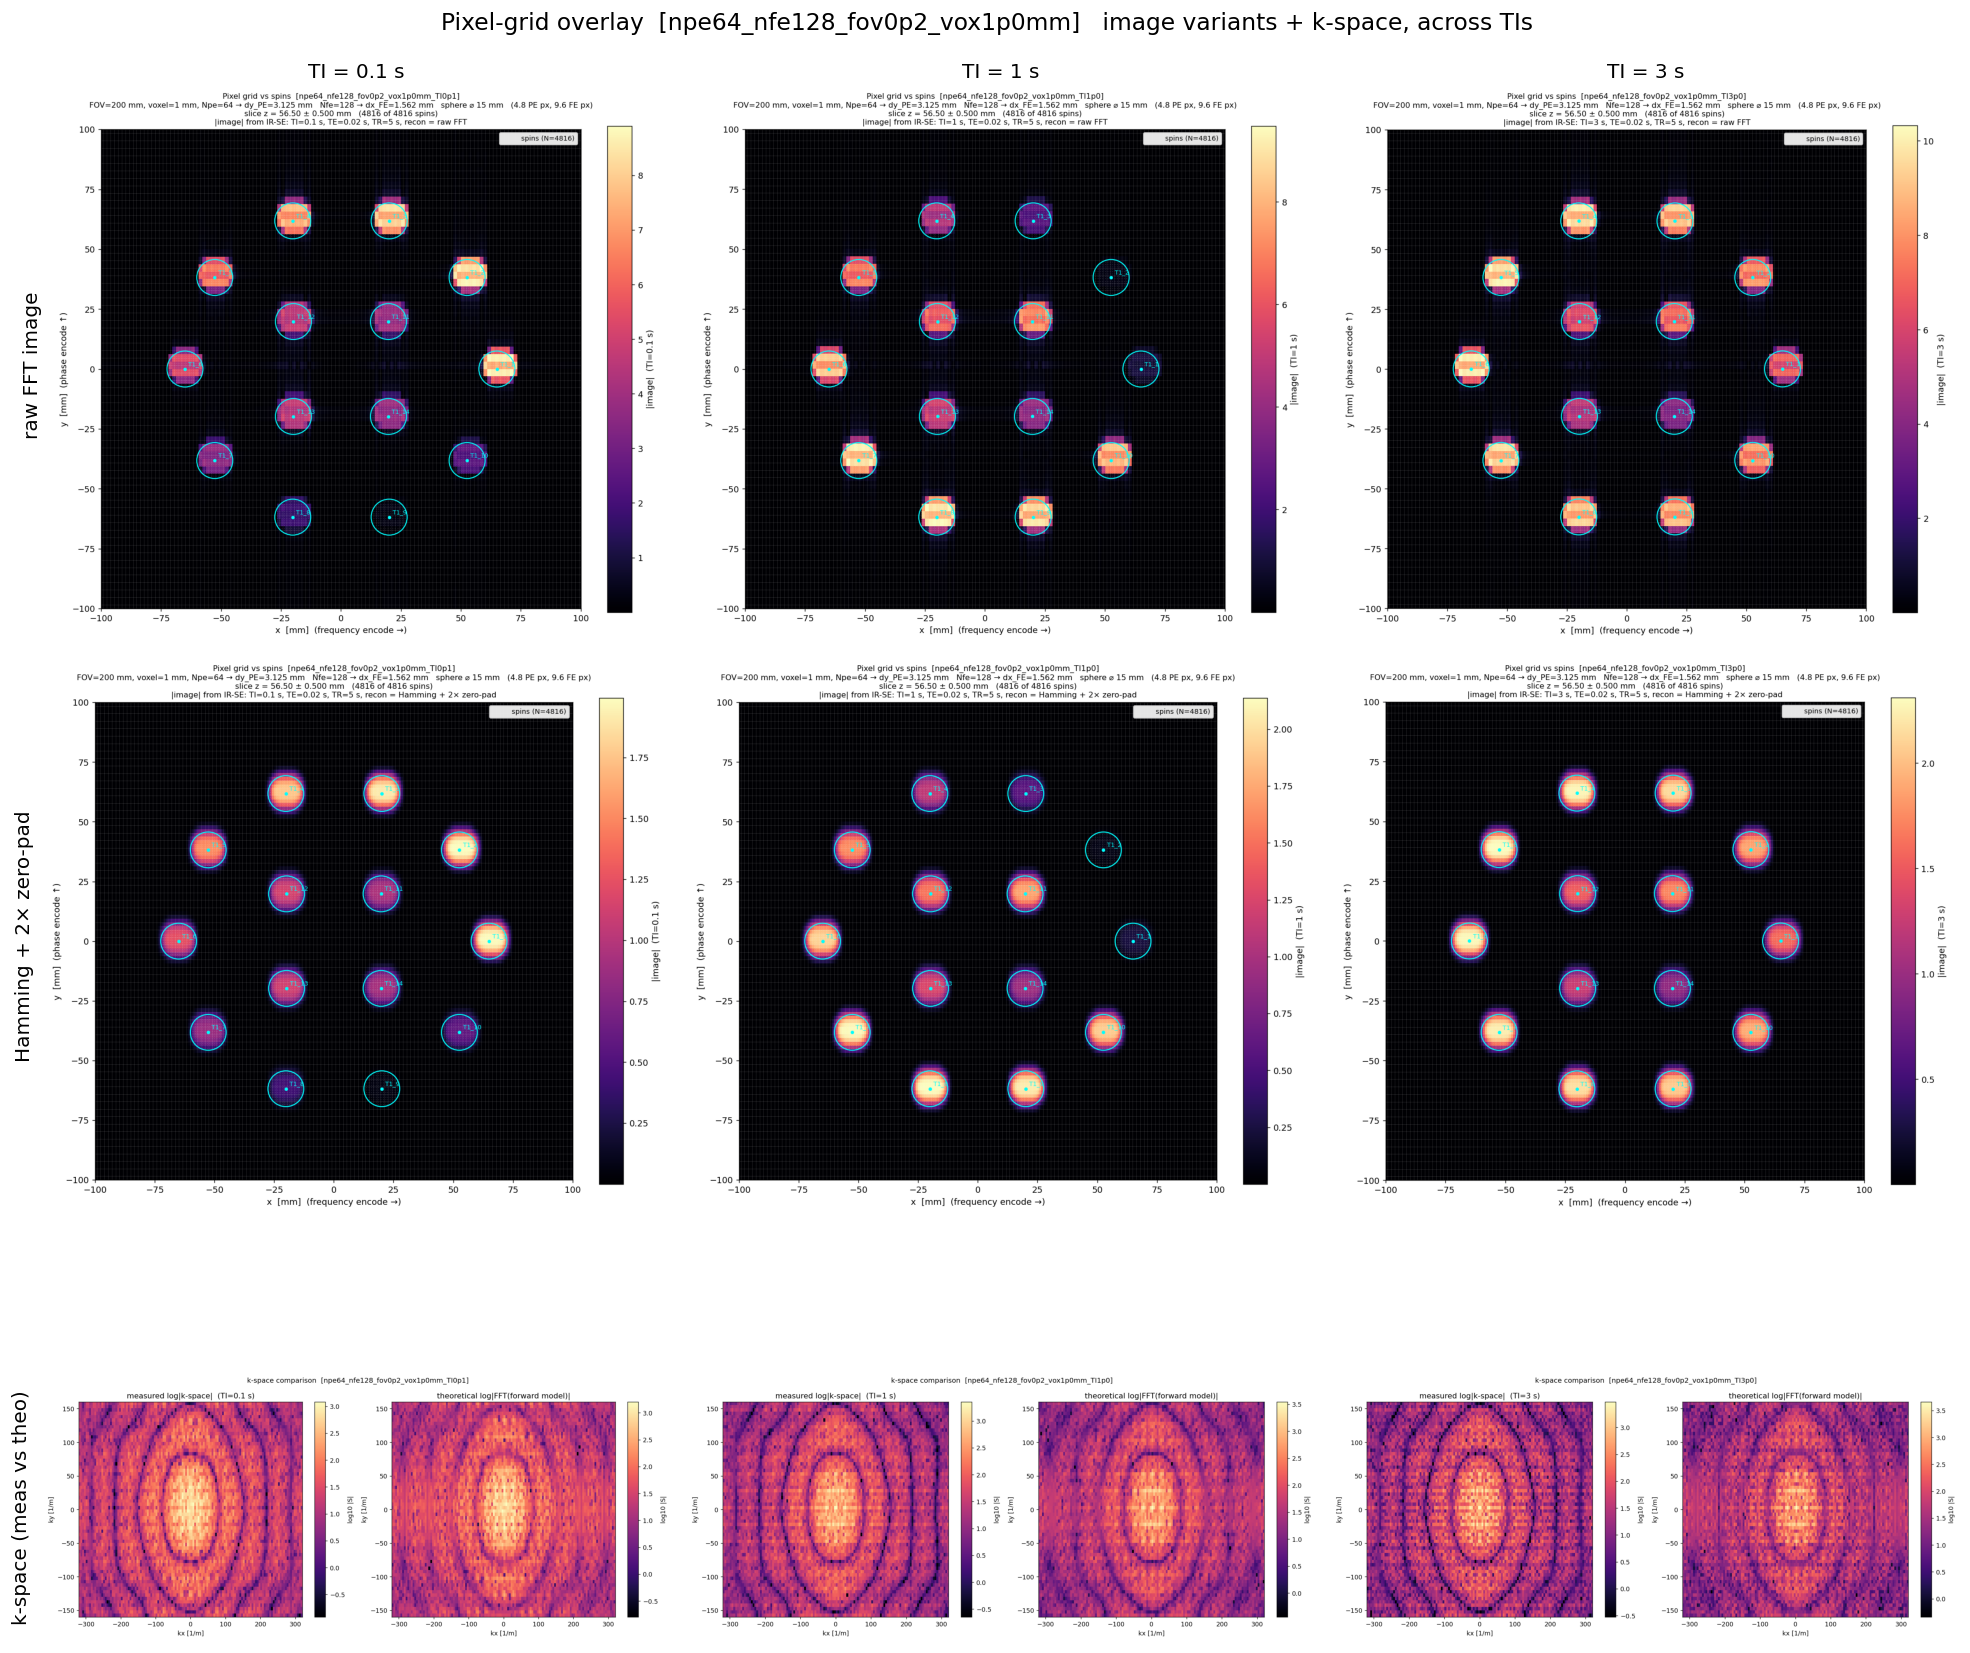
\includegraphics[width=0.82\linewidth]{imgs/komaMRI/fixed_pixel_grid_overlay.png}
\captionof{figure}{Reconstructed images after both fixes. The spheres remain
well-localised across the full phase-encode direction. The time-dependent
streaking in Figure~\ref{fig:komamri-buggy-pixel-grid} is removed.}
\label{fig:komamri-fixed-pixel-grid}
\end{center}

\begin{center}
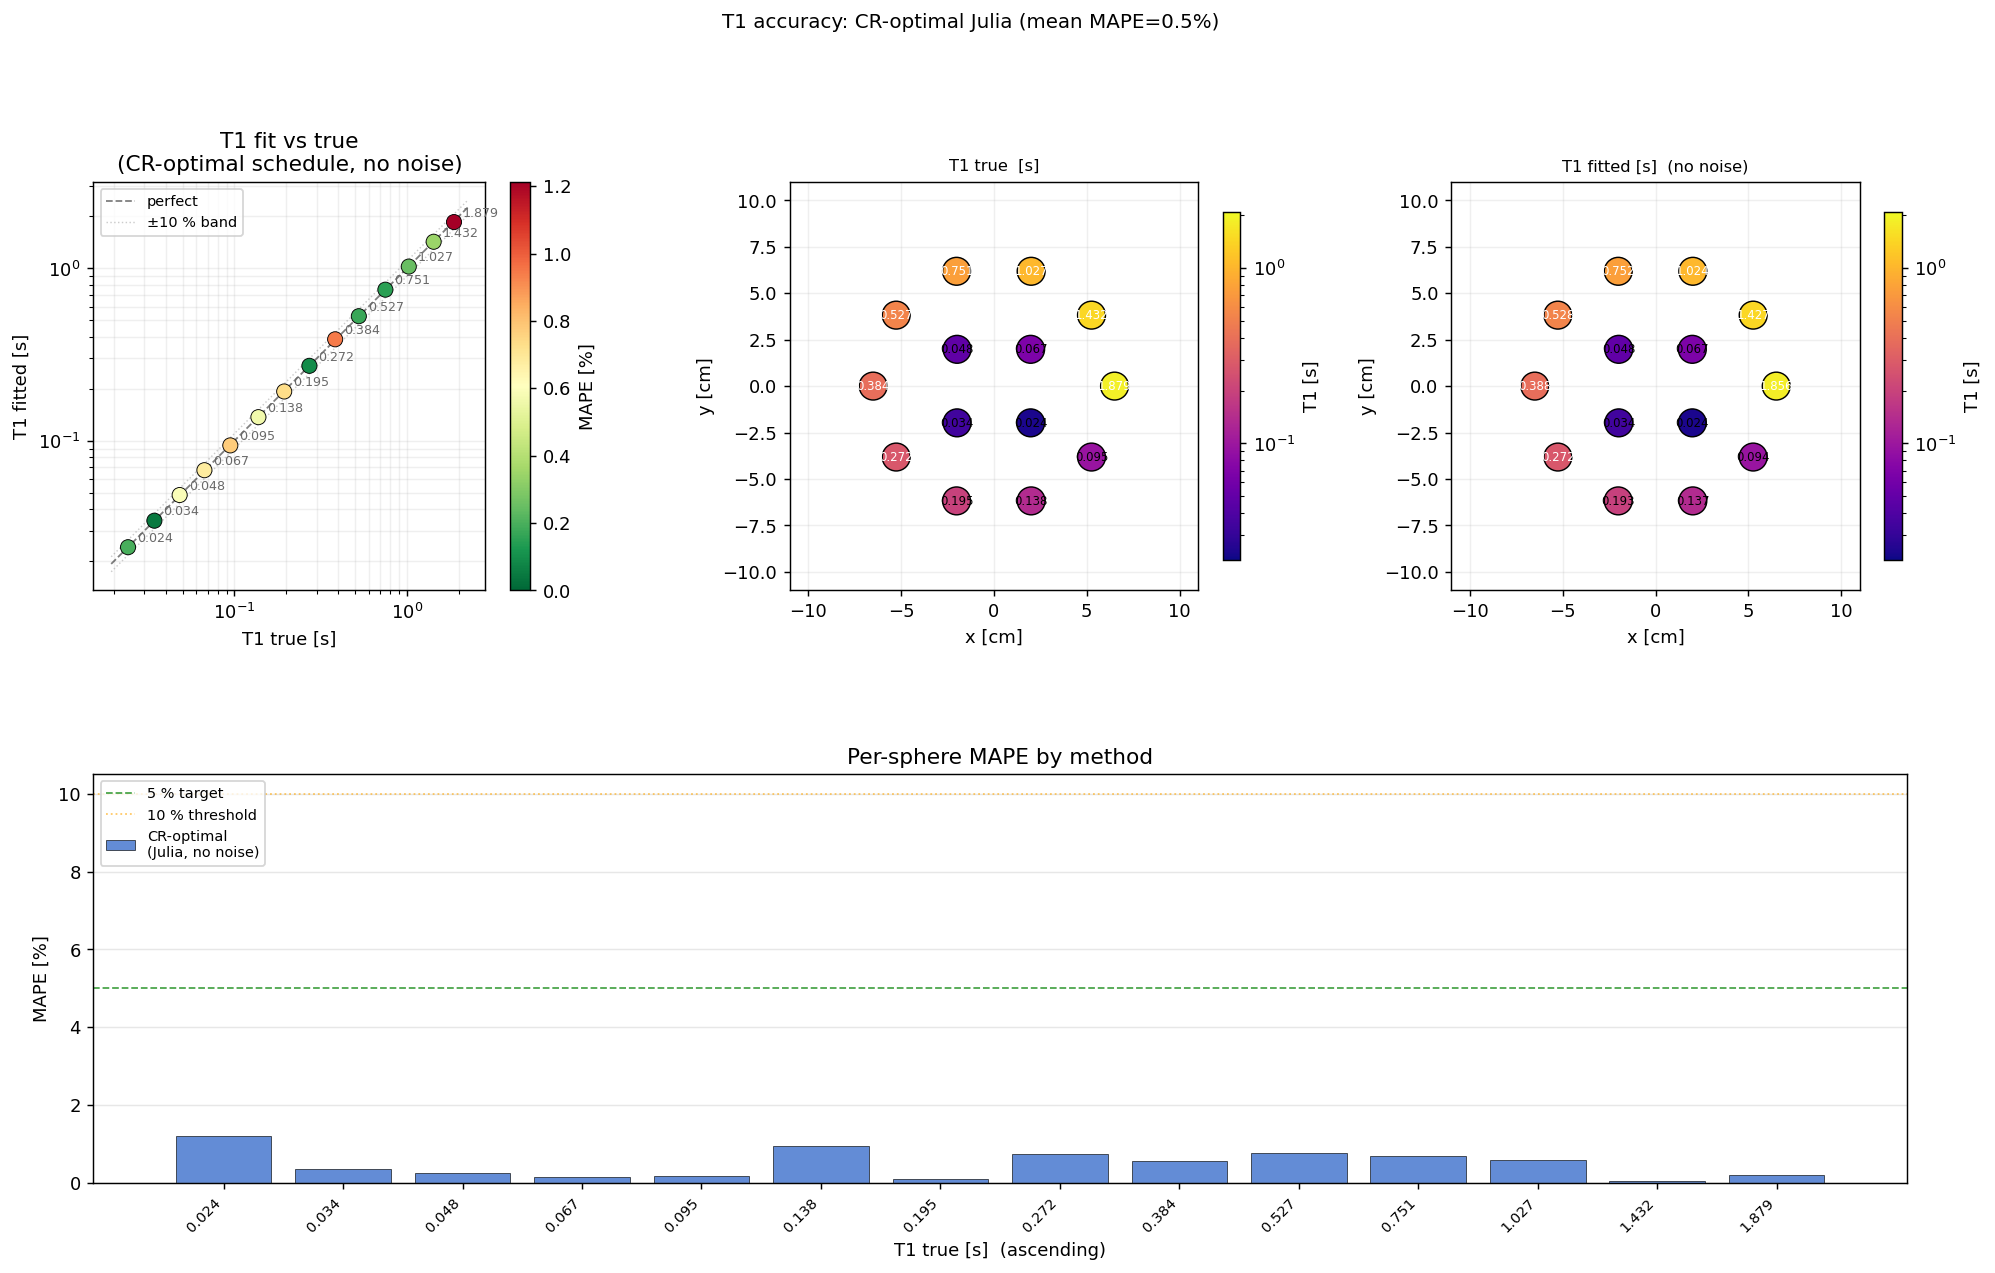
\includegraphics[width=0.62\linewidth]{imgs/komaMRI/fixed_t1_fit_vs_true.png}
\captionof{figure}{Noise-free $T_1$ recovery after both fixes. Mean MAPE decreases from
39.4\% to 0.48\%, and all spheres are within 1.21\% of their true value. This
is the expected accuracy for the noise-free validation case.}
\label{fig:komamri-fixed-t1-fit}
\end{center}

\begin{center}
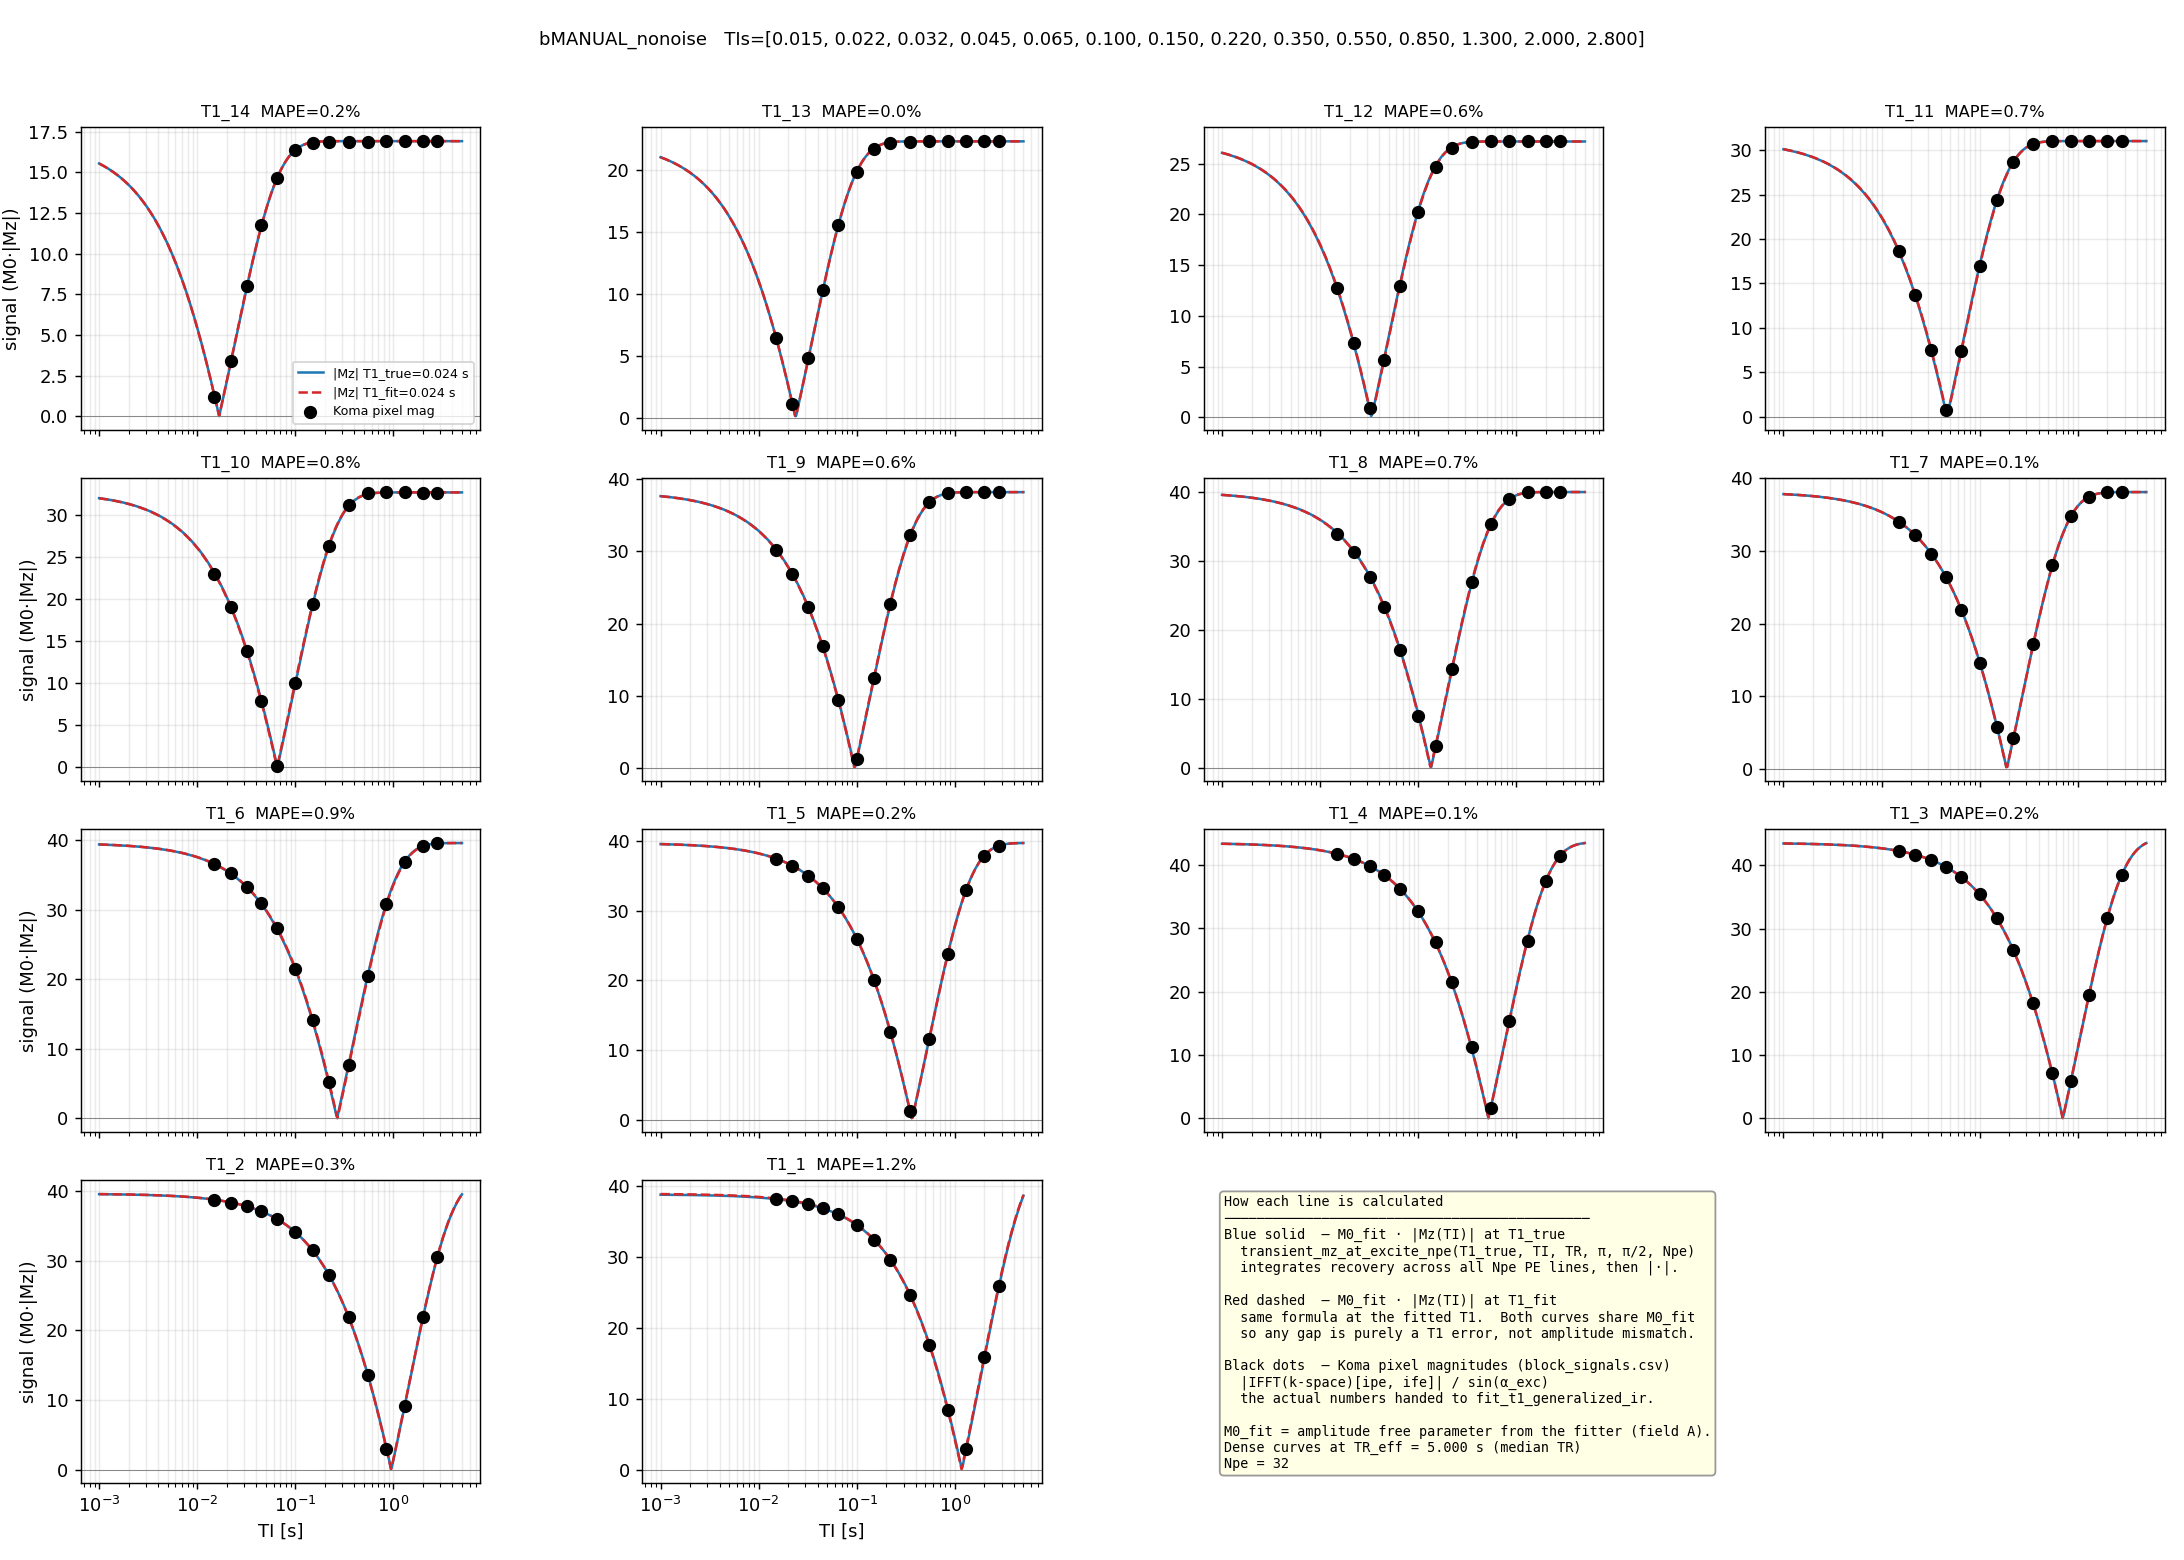
\includegraphics[width=0.68\linewidth]{imgs/komaMRI/fixed_recovery_curves_koma.png}
\captionof{figure}{Recovery curves after both fixes. The simulated samples now lie on the
fitted inversion-recovery curves.}
\label{fig:komamri-fixed-recovery-curves}
\end{center}

\FloatBarrier

\section{Evaluation of the fixes}
\label{sec:komamri-fix-evaluation}

The fixes were evaluated at multiple levels, from isolated timing behaviour to
the full qMRI validation task.

\begin{center}
\begingroup
\small
\setstretch{1}
\setlength{\tabcolsep}{3pt}
\renewcommand{\arraystretch}{1.08}
\begin{tabularx}{\linewidth}{%
  >{\raggedright\arraybackslash}p{0.17\linewidth}
  >{\raggedright\arraybackslash}p{0.25\linewidth}
  >{\raggedright\arraybackslash}X
  >{\raggedright\arraybackslash}X}
\toprule
Level & Test & Before fix & After fix \\
\midrule
Timing representation & RF-edge discretisation at large absolute time &
RF edge markers collapse once cumulative time reaches the 70--150 s regime &
Stable to 1000 s \\
Minimal signal reproducer & Identical IR shots, no gradients
(\texttt{koma\_bug\_minimal.jl}) & 19--21\% signal jump once cumulative time
reaches 72--120 s & Flat over tested shots \\
Residual timing reproducer & 24 identical IR shots, no gradients
(\texttt{koma\_bug\_residual.jl}) & +52\% jump at shot 18 (270 s), then wrong
plateau & Flat over all 24 shots \\
Full qMRI validation & No-noise 14-sphere $T_1$ recovery & 39.4\% mean MAPE &
0.48\% mean MAPE (1.2\% max MAPE) \\
Regression safety & KomaMRI test suite & New timing tests fail on unfixed code &
Passes after both fixes \\
\bottomrule
\end{tabularx}
\captionof{table}{Summary of KomaMRI timing-fix validation.}
\label{tab:komamri-fix-evaluation}
\endgroup
\end{center}

The minimal reproducers show that the specific floating-point failures were
removed, while the phantom validation shows that the corrected simulator
produces accurate quantitative maps.

\subsection{Why this mattered for qMRI}
\label{subsec:komamri-why-qmri}

The timing failure had likely gone unnoticed because it is triggered by long cumulative
sequence time, while most examples and tests are much shorter, never reaching
the $\sim128$ s absolute-time regime where Float64 spacing becomes comparable
to the fixed $\epsilon$ marker. This threshold is still well within the
duration of many clinical MRI acquisitions, which often last several minutes.
The largest effect also appears for hard RF pulses with sharp edges: losing one
$\Delta t_\mathrm{rf}$ sample is a large fraction of a 1 ms rectangular pulse.
In practical slice-selective sequences, shaped RF pulses and gradient ramps
make the same timing error a smaller perturbation.

A second reason is that most MRI simulation checks are qualitative: a
reconstructed image can still look plausible when noise and contrast variation
hide small systematic signal errors. qMRI is stricter. The validation compares
fitted $T_1$ values against known phantom ground truth, so a systematic signal
error directly appears as parameter bias. This project exposed the failure because
RL training needs long sequences and qMRI validation needs quantitative
agreement, not just plausible images.

This validation covers the IR-SE sequence family used for the main experiments;
other sequence families would require the same timing and no-noise recovery
checks before being used for quantitative claims.

\subsection{Why spoiling was a convincing false lead}
\label{subsec:komamri-spoiling-false-lead}

Although presented here as a single validation narrative, the investigation
happened in two stages. Before either fix, transverse spoiling looked plausible
because it reduced the catastrophic 924.5\% MAPE failure to 92.6\%, suggesting
that residual transverse magnetisation might be part of the problem. After the
first timing failure was fixed, the remaining error was smaller, around 30--40\%, and
therefore more consistent with a possible sequence effect. Spoiling had to be
rechecked before the second timing bug was isolated. In the intermediate
simulator shown in Figures~\ref{fig:komamri-buggy-t1-fit} to
\ref{fig:komamri-buggy-pixel-grid}, however, spoiling increased mean MAPE from
39.4\% to 44.0\%. After both fixes, spoiled and unspoiled no-noise fits are
both sub-percent (0.43\% and 0.48\% mean MAPE respectively). Spoiling remains
important for realistic sequence design, but it was not the cause of this
validation failure.
